%!TEX TS-program = xelatex
%!TEX encoding = UTF-8 Unicode

%%
%% 使用 njuthesis 文档类生成南京大学本科生毕业论文的示例文档
%% 
%%

%% 
%% 南京大学本科学位论文模板
%% 2018年封面,摘要都发生了变化,本模板由以下2016年模板更改而来:http://haixing-hu.github.io/nju-thesis/

%% 如需Adobe字体请用(默认)
%\documentclass[adobefonts]{njuthesis}
%% MacOS系统请用
%\documentclass[macfonts]{njuthesis}
%% Windows系统请用
\documentclass[winfonts]{njuthesis}
%\usepackage{enumerate}
\usepackage{enumitem}
%% Linux系统请用
%\documentclass[linuxfonts]{njuthesis}
\newcommand\redbf[1]{\textbf{\textcolor{red}{#1}}}
\renewcommand{\today}{\number\year 年 \number\month 月 \number\day 日}
%%%%%%%%%%%%%%%%%%%%%%%%%%%%%%%%%%%%%%%%%%%%%%%%%%%%%%%%%%%%%%%%%%%%%%%%%%%%%%%
% 设置论文的中文封面
% 论文标题
\title{安卓不可见控件内存泄漏的自动检测}

% 论文作者姓名
\author{王冬杨}
% 论文作者学号
\studentid{161250136}
% 导师姓名职称
\supervisor{马骏}
% 导师职称
\supervisortitle{副教授}
% 论文作者院系
\department{软件学院}
% 论文作者专业方向
\major{软件工程}
% 论文作者的年级
\grade{2016级}
% 论文提交日期,需设置年、月、日。此属性可选,默认值为最后一次编译时的日期,精确到日。
\submitdate{\today}

%%%%%%%%%%%%%%%%%%%%%%%%%%%%%%%%%%%%%%%%%%%%%%%%%%%%%%%%%%%%%%%%%%%%%%%%%%%%%%%
% 设置论文的英文封面

% 论文的英文标题
\englishtitle{Thesis paper template}
% 论文作者姓名的拼音
\englishauthor{San Zhang}
% 导师姓名职称的英文
\englishsupervisor{Professor Si Li}
% 论文作者所在院系的英文名称
\englishdepartment{School of Electronic Science and Engineering}
% 论文作者所在学校或机构的英文名称。此属性可选,默认值为``Nanjing University''。
\englishinstitute{Nanjing University}
% 论文完成日期的英文形式,默认最后一次编译的时间
\englishdate{May 20, 2018}
% 专业
\englishinstitute{Electronic Information Science and Technology}
%%%%%%%%%%%%%%%%%%%%%%%%%%%%%%%%%%%%%%%%%%%%%%%%%%%%%%%%%%%%%%%%%%%%%%%%%%%%%%%
% 设置论文的页眉页脚
\usepackage{fancyhdr}
%\usepackage{enumitem}

\pagestyle{fancy}
%\lhead{\bfseries 141180092 }
\chead{安卓不可见控件内存泄漏的自动检测}
\rhead{王冬杨}
%\lfoot{From: K. Grant}
%\cfoot{To: Dean A. Smith}
%\rfoot{\thepage}
\renewcommand{\headrulewidth}{0.4pt}
%\renewcommand{\footrulewidth}{0.4pt}
%%%%%%%%%%%%%%%%%%%%%%%%%%%%%%%%%%%%%%%%%%%%%%%%%%%%%%%%%%%%%%%%%%%%%%%%%%%%%%%

\usepackage{xcolor}
\usepackage{minted}

\usepackage{listings}

\usepackage{color}
\definecolor{gray}{rgb}{0.4,0.4,0.4}
\definecolor{darkblue}{rgb}{0.0,0.0,0.6}
\definecolor{cyan}{rgb}{0.0,0.6,0.6}

\lstset{
	basicstyle=\ttfamily,
	columns=fullflexible,
	showstringspaces=false,
	commentstyle=\color{gray}\upshape
}
\begin{document}

% 制作中文封面
\maketitle
% 制作英文封面
% \makeenglishtitle
% 毕业论文过程管理四页表
% \controlpage %可以将word文件交给老师签字后扫描转成pdf,然后命名为controlpage.pdf

% 论文的中文摘要
\begin{abstract}

在安卓应用中,服务和广播得到了广泛应用,提供诸如下载,数据更新,跨应用通信等功能。但由于开发者经常忽视这些不可见控件的生命周期管理,因此内存泄漏发生的几率很高。

本文将会关注新版本安卓系统(Android 8+)中公开服务(Exported Services)以及静态注册的广播接收器的内存泄露问题,阐述公开服务和广播接收器内存泄露的检测方法,并编写一套供服务开发人员使用的自动分析组件内存泄露的检测工具,最后会从应用市场(App Store)中下载真实的应用,进行内存泄漏检测和分析。

% 同时应该注意到,空白页是故意留白,以便章节开头能够出现在偶数页。
% 中文关键词。关键词之间用中文全角分号隔开,末尾无标点符号。
\keywords{安卓系统;内存泄漏;安卓服务;安卓广播}
\end{abstract}

%%%%%%%%%%%%%%%%%%%%%%%%%%%%%%%%%%%%%%%%%%%%%%%%%%%%%%%%%%%%%%%%%%%%%%%%%%%%%%%
% 论文的英文摘要
% \begin{englishabstract}
% The diversity of handwritten Chinese text make it a promising but % challenging computer vision problem. 
% 英文关键词。关键词之间用英文半角逗号隔开,末尾无符号。
% \englishkeywords{Handwritten Chinese, Text recognition, Deep learning}
% \end{englishabstract}

%%%%%%%%%%%%%%%%%%%%%%%%%%%%%%%%%%%%%%%%%%%%%%%%%%%%%%%%%%%%%%%%%%%%%%%%%%%%%%%
% 论文的前言,应放在目录之前,中英文摘要之后
%
%\begin{preface}
%
%在过去的40年中,手写中文文本领域识别(HCTR)取得了很大的进展[1,2]。
%
%\vspace{1cm}
%\begin{flushright}
%饶安逸\\
%2018年5月15日于南大仙林
%\end{flushright}
%
%\end{preface}

%%%%%%%%%%%%%%%%%%%%%%%%%%%%%%%%%%%%%%%%%%%%%%%%%%%%%%%%%%%%%%%%%%%%%%%%%%%%%%%
% 生成论文目录
\tableofcontents

%%%%%%%%%%%%%%%%%%%%%%%%%%%%%%%%%%%%%%%%%%%%%%%%%%%%%%%%%%%%%%%%%%%%%%%%%%%%%%%
% 生成插图清单。如无需插图清单则可注释掉下述语句。
%\listoffigures

%%%%%%%%%%%%%%%%%%%%%%%%%%%%%%%%%%%%%%%%%%%%%%%%%%%%%%%%%%%%%%%%%%%%%%%%%%%%%%%
% 生成附表清单。如无需附表清单则可注释掉下述语句。
%\listoftables

%%%%%%%%%%%%%%%%%%%%%%%%%%%%%%%%%%%%%%%%%%%%%%%%%%%%%%%%%%%%%%%%%%%%%%%%%%%%%%%
% 开始正文部分
\mainmatter

%%%%%%%%%%%%%%%%%%%%%%%%%%%%%%%%%%%%%%%%%%%%%%%%%%%%%%%%%%%%%%%%%%%%%%%%%%%%%%%
% 学位论文的正文应以《绪论》作为第一章
\chapter{绪论}\label{chapter_introduction}
\section{研究背景}
在安卓应用中,服务(Services)和广播(Broadcast)得到了广泛的使用。服务可以在安卓应用的后台保持长期运行,提供诸如下载、数据更新等重要功能。然而,正因为服务长期运行于后台的特点,使其往往容易产生异常(Errors)。如果服务的编写人员缺少警惕性,服务中出现的错误(Bug)可能会导致诸多问题,严重者可能引起应用崩溃,甚至系统死机;广播是一种常被用来进行跨应用的通信的通信手段,应用在使用广播进行与系统或者与其他应用进行通讯时,应用需要编写广播接收器(Broadcast Receiver)。负责运行广播接收器的时应用的主线程种,因此在广播接收器中不适合进行耗时操作,通常会在广播接收器中启动服务来进行后续的处理,因此广播接收器也可能通过服务或者自身导致内存泄漏。

安卓应用中的内存泄露指资源(内存对象、句柄、服务等)将不再被使用,但却无法被安卓系统的垃圾回收器(Garbage Collector)所回收,同时也是服务中的一大类常见问题。服务如果出现内存泄露,将会导致内存使用量意外大幅度增加,进而使得系统效率降低,严重影响用户体验。

有一类服务被称为\textbf{公开服务},即指定了\textbf{"exported:true"}属性的服务。其他应用在满足一定条件时(满足权限要求等)可以启动应用的公开服务,因此内存泄露的问题将会变得更加复杂。

由于在安卓8及更高的版本下,安卓操作系统的“电池优化策略”禁止跨应用启动后台服务\cite{android-service-limit},而这一方式在安卓7以及更早的版本中是可行的,因此在新版本(安卓8及更高)的安卓系统中,公开服务的内存泄漏检测方法与之前的方法\cite{jun2018lesdroid}有所差别,也正因为禁止跨应用启动后台服务,公开服务的内存泄漏问题也得到了很大的规避。

\section{相关工作}

Erika 等人在安卓8之前的版本中,编写了一个检测跨应用通信安全问题的工具Com Droid\cite{chin2011analyzing},文中阐述的方法对于跨应用测试具有指导意义。


在安卓8之前的版本中,跨应用启动服务这一行为是被允许的,南京大学的马骏等人安卓8之前的版本中,实现过一个公开服务(Exported Services)内存泄漏的检测工具LES Droid\cite{jun2018lesdroid},文中采用的方式分为四步:

\begin{enumerate}
	\item 使用apktool反编译工具\cite{apktool}对被测试应用进行反编译,获取被测试应用的安卓组件清单(AndroidManifest.xml)文件,解析获取应用中所有的公开服务的包名和类名。
	\item 将测试驱动应用、被测试应用通过adb安装到模拟器中,启动测试驱动应用。
	\item 测试驱动应用重复启动、关闭被测试的服务,在满足一定测试强度之后,导出被测试应用的堆镜像文件(.hprof files)。
	\item 基于MAT内存分析库\cite{mat}编写堆镜像文件的分析工具,自动检测内存泄漏并统计泄露的入口等。
\end{enumerate}

\label{pre-result}
文中的数据指出:在41537个被测试应用中,共在其中28662(69\%)个应用中检测出74831个服务,其中3934(13.7\%)个应用拥有公开服务。经过去重、安装测试以及应用商店评分筛选,有375个实际测试应用,最终通过不同的测试配置,最终检测到在18.7\%的应用中有16.8\%的服务存在内存泄漏问题。


\section{本文主要工作}
本文旨在探索一套适用于安卓8以上版本的公开服务和静态注册广播接收器的内存泄漏检测方法。主要工作如下:
\begin{enumerate}
\item 找到在安卓8以上版本的安卓系统上可行的跨应用测试方法。

\item 对桩应用上进行测试,并能发现所有泄露。

\item 在应用商店中下载真实应用,进行自动化测试分析实验结果。

\end{enumerate}
\section{本文结构}
本文的各章节组织结构如下:
\begin{itemize}
	\item[第一章] 绪论。简要说明了安卓组件内存泄漏的现象和后果。并概括地描述了检测安卓不可见控件内存泄漏的方法流程,总结了本文结构。
	\item[第二章] 背景
	\item[第三章] 自动化检测工具。
	\item[第四章] 实验。介绍了实验进行的配置环境,测试使用应用的来源,以及实验数据结果。
	\item[第五章] 总结与讨论。总结全文工作,讨论存在的问题和今后可以继续研究的方向。
\end{itemize}

\chapter{自动化检测工具}\label{chapter_system}

本章将介绍安卓控件启动的流程,及检测内存泄露的原理。

\section{安卓服务}
安卓应用中的服务可以通过两种方式启动\cite{service}:

\textbf{start 方式 } 其他组件构造特定的\textbf{Intent}对象,通过调用\textbf{startService() API}来启动目标服务。

\textbf{bind 方式 } 通过调用\textbf{bindService() API}将目标服务与特定组件绑定。被绑定的服务提供接口供其他组件与之交互。
一个服务可以同时通过以上两种方式启动。

\subsection{服务的生命周期}
服务的生命周期根据启动方式不同分为两种\cite{service}:

\textbf{start 方式 } 通过\textbf{startService() API}启动的服务将会一直运行,直到调用\textbf{stopSelf()}方法将自己停止运行。其他组件也可以通过调用\textbf{stopService() API}将服务停止运行。

停止运行的服务将会被\textbf{GC(Garbage Collector)}回收。

\textbf{bind 方式 } 通过\textbf{bindService() API}启动的服务将通过\textbf{IBinder}接口与其他组件进行交互,直到其他组件调用\textbf{unbindService() API}解除绑定。

一个服务可以同时绑定到多个组件之上,直到所有组件都解除了绑定时,该服务才会被\textbf{GC}回收。

每个安卓应用都关联一个\textbf{ActivityThread}实例,负责调度和执行该应用的各种组件。\textbf{ActivityThread}有一个\textbf{ArrayMap}类型的成员变量\textbf{mServices},其中保存了所有没有被销毁的服务的引用。一旦某个服务的实例被销毁,其引用将会从\textbf{mServices}中删除。

\subsection{服务的注册方式}
\begin{listing}[htbp]
	\centering
	\caption{服务的注册方式}
	\begin{minted}[encoding=utf8,
	frame=single,
	framesep = 1em,
	numbers=left, 
	breaklines=true, 
	tabsize=4,
	xleftmargin=2em,xrightmargin=2em,
	fontsize=\footnotesize]{xml}
<manifest
    xmlns:android="http://schemas.android.com/apk/res/android"
    xmlns:dist="http://schemas.android.com/apk/distribution"
    package="com.example.myapplication">
    <dist:module dist:instant="true" />
    <application ...>
        ...
        <service android:name=".Service1"
            android:enabled="true"
            android:exported="true">
        </service>
        <service
            android:name = ".Service2"
            android:enabled = "true"
            android:exported = "false">
            <intent-filter>
                <category android:name = "cat1"/>
                <action android:name = "act2"/>
            </intent-filter>
        </service>
        <service android:name = ".Service3"
            android:enabled = "true"
            android:permission = "Permission1">
            <intent-filter>
                <action android:name = "act3"/>
                <category android:name = "cat2"/>
                <data android:scheme = "Scheme1"/>
                <data android:scheme = "Scheme2"/>
            </intent-filter>
        </service>
    </application>
</manifest>
	\end{minted}
	\label{declaration:service}
\end{listing}
通常,每个服务都要在\textbf{AndroidManifest.xml}中注册一个\textbf{<service>}标签(参考Listing.\textcolor{red}{\ref{declaration:service}}中的样例)。同时服务可以通过设置"\textbf{android:exported}"属性来指定该服务是否将被导出。当设置\textbf{android:exported = "true"}时,该服务可以被其他应用使用,反之不可。
%可以凑更多字数
\subsection{服务的内存泄漏}\label{service_leak}
通常,一个服务的实例不再被使用时应该被\textbf{GC(Garbage Collector)}回收,并释放资源。然而在某些情况下,一个被销毁的服务可能会意外的被引用,从而使得\textbf{GC}无法将其回收并释放资源,这样就造成了服务的内存泄漏。
\begin{listing}[htbp]
	\centering
	\caption{服务的内存泄漏}
	\begin{minted}[encoding=utf8,
		frame=single,
		framesep = 1em,
		numbers=left, 
		breaklines=true, 
		tabsize=4,
		showtabs = false,
		xleftmargin=2em,xrightmargin=2em,
		fontsize=\footnotesize]{java}
public class LeakedService extends Service{
	private static final String TAG = "LeakedService";
	// Method will be called when an instance is creating.
	public void onCreate(){
		...
		new Timer().scheduleAtFixedRate(new TimerTask(){
			public void run(){
				Log.d(TAG, LeakedService.this.getPackageName() + ".LeakedService is running!");
			}
		},1000L,3000L);
	}
	// Method will be called when an instance is destroying.
	public void onDestroy(){
		...
	}
}
	\end{minted}
	\label{leaked example:service}
\end{listing}

例如在游戏\emph{com.siendas.games2048}中,就出现了原理如图(见\textbf{Listing.\textcolor{red}{\ref{leaked example:service}}})的内存泄漏。具体导致内存泄露的原理为:在\textbf{LeakedService}的实例被构造的时候,将会调用他的\textbf{onCreate()}方法,在该方法中延迟\textbf{1000ms}启动了一个\textbf{匿名}计时器,该计时器将以\textbf{3000ms}的周期打印调试信息,可以看到在\textbf{TimerTask}类中持有了\textbf{LeakedService}的引用,而在该服务被销毁时,其\textbf{onDestroy()}方法中并没有对该匿名计时器进行销毁。因此在该服务被销毁后,将会一直存在一个匿名计时器持有该服务的引用,导致\textbf{GC}无法将其回收,从而导致了内存泄漏。

\section{安卓广播接收器}
安卓应用中的广播接收器亦有两种方式启动\cite{broadcast}:

\textbf{清单声明的接收器 }\label{declaration:receiver in manifest} 通过在\textbf{AndroidManifest.xml}中添加\textbf{<receiver>}标签注册广播接收器,通过\textbf{<intent-filter>}标签指定接收器所订阅的广播操作。系统软件包管理器会在应用安装时注册接收器。然后,该接收器会成为应用的一个独立入口点,这意味着如果应用当前尚未运行,系统可以启动应用并发送广播。系统会创建新的\textbf{BroadcastReceiver}组件对象来处理它接收到的每个广播。次对象仅在调用\textbf{onReceive(Context, Intent)}期间有效。一旦从此方法返回代码,系统便会认为该组件不再活跃。

\textbf{上下文注册的接收器 }\label{declaration:receiver in context} 通过在代码中构造出\textbf{BroadReceiver}实例,以及\textbf{IntentFilter}实例来指定订阅的广播内容,调用\textbf{registerReceiver(BroadcastReceiver, IntentFilter) API}来注册接收器。只要上下文有效,通过改种方式注册的广播接收器就会接收广播。如果要停止接收广播,需要调用\textbf{unregisterReceiver(BroadcastReceiver) API}来注销广播接收器

\subsection{广播接收器的生命周期}
广播接收器的生命周期根据启动方式不同亦分为两种\cite{broadcast}:

\textbf{清单声明的接收器 } 静态注册的接收器生命周期不限于\textbf{Activity}甚至整个应用。即使应用并不在运行,接收器也可以接收到订阅的广播。将会在\textbf{onReceive()}方法结束后被销毁。


\textbf{上下文注册的接收器 } 上下文注册的接收器,其生命周期仅限于注册的上下文,例如在\textbf{Activity}上下文注册的接收器,在整个\textbf{Activity}存活期间可以持续接收广播;在应用上下文中注册的接收器,则会在整个应用运行期间都可以接收广播。需要注意的是:这种方式启动的接收器必须手动进行销毁,即调用\textbf{unregisterReceiver() API},否则在上下文失效时,系统会抛出异常(并不会导致应用崩溃),同时接收器会引发泄露(见图.\textcolor{red}{\ref{fig:broadcast_leak}})。

\begin{figure}[htbp]
   \centering
   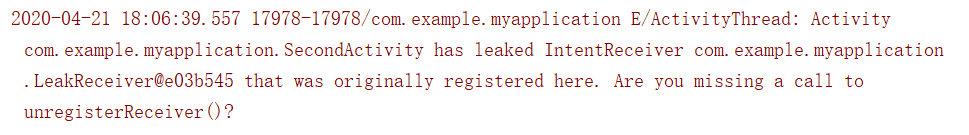
\includegraphics[width=0.9\textwidth]{broadcast_leak.png} % requires the graphicx package
   \caption{没有回收接收器将会导致异常以及泄露}
   \label{fig:broadcast_leak}
\end{figure}

\subsection{广播接收器的注册方式}
\begin{listing}[htbp]
	\centering
	\caption{广播接收器的注册方式}
	\begin{minted}[encoding=utf8,
	frame=single,
	framesep = 1em,
	numbers=left, 
	breaklines=true, 
	tabsize=4,
	showtabs = false,
	xleftmargin=2em,xrightmargin=2em,
	fontsize=\footnotesize]{XML}
<manifest 
	xmlns:android="http://schemas.android.com/apk/res/android"
	xmlns:dist="http://schemas.android.com/apk/distribution"
	package="com.example.myapplication">
	<dist:module dist:instant="true" />
	<application ...>
		...
		<receiver
			android:name = ".Receiver1">
			<intent-filter>
				<action android:name = "act1" />
			</intent-filter>
		</receiver>
		<receiver
			android:name = ".Receiver2"
			android:exported = "false"
			android:enabled = "true">
			<intent-filter>
				<category android:name = "cat1" />
				<action android:name = "act2" />
			</intent-filter>
		</receiver>
	</application>
</manifest>
	\end{minted}
	\label{declaration:receiver}
\end{listing}

一般而言,清单声明的广播接收器(见\ref{declaration:receiver in manifest})需要在\textbf{AndroidManifest.xml}文件中添加\textbf{<receiver>}标签(参考\textbf{Listing.\textcolor{red}{\ref{declaration:receiver}}}),在\textbf{<intent-filter>}子标签中可以指定订阅的广播内容等,也可以通过设置\textbf{"android:exported"}属性来指定该广播是否将被导出。而上下文注册的广播接收器(见\ref{declaration:receiver in context})则不需要进行前文的操作。
\subsection{广播接收器的内存泄漏}
广播接收器的内存泄漏原理类似与服务内存泄漏\ref{service_leak}。但是由广播接收器引起的内存泄漏往往比服务更为严重,因为广播接收器被系统认为只进行不耗时的操作(如果超过10s未从\textbf{onReceive()}方法中返回,将抛出\textbf{ANR Exception}),因此通常广播接收器在接到广播后,很有可能会启动其他的\textbf{Service}进行后续的耗时操作,进而可能会导致一连串的内存泄漏。

例如图中(见\textbf{Listing.\textcolor{red}{\ref{leaked example:receiver}}})所示的广播接收器,不仅本身会导致内存泄漏,而且还会启动一个会导致内存泄漏的服务(见\textbf{Listing.\textcolor{red}{\ref{leaked example:service}}}),因此后果将会更加严重。
\begin{listing}[htbp]
	\centering
	\caption{广播接收器的内存泄漏}
	\begin{minted}[encoding=utf8,
	frame=single,
	framesep = 1em,
	numbers=left, 
	breaklines=true, 
	tabsize=4,
	showtabs = false,
	xleftmargin=2em,xrightmargin=2em,
	fontsize=\footnotesize]{java}
public class LeakReceiver extends BroadcastReceiver {
	private final String TAG = "LeakReceiver";
	private final int ID = new Random().nextInt();
	@Override
	public void onReceive(Context context, Intent intent) {
		...
		context.startService(new Intent(context,LeakService.class));
		new Timer().scheduleAtFixedRate(new TimerTask() {
			@Override
			public void run() {
				Log.i(TAG,LeakReceiver.this.ID + " is running!");
			}
		}, 1000L, 3000L);
	}
}
	\end{minted}
	\label{leaked example:receiver}
\end{listing}
\section{自动化检测工具原理}



\chapter{总结与讨论}
在本文中,我们使用预处理层-卷积层-循环卷积层-转录层网络来处理手写中文文本识别的问题。这种网络很好地结合了卷积网络和循环网络各自的优势。

\bibliography{sample}

%%%%%%%%%%%%%%%%%%%%%%%%%%%%%%%%%%%%%%%%%%%%%%%%%%%%%%%%%%%%%%%%%%%%%%%%%%%%%%%
% 致谢,应放在结论之后
\begin{acknowledgement}
感谢在实验室度过的两年时光,老师无论在学术还是人生的指导上都对我起到了很大的帮助;师兄师姐小伙伴们的鼓励支持和陪伴是我坚持下去的动力。
\end{acknowledgement}

%%%%%%%%%%%%%%%%%%%%%%%%%%%%%%%%%%%%%%%%%%%%%%%%%%%%%%%%%%%%%%%%%%%%%%%%%%%%%%%
\end{document}
